\section{Il Progetto IEEE 802}

Il progetto \textbf{IEEE 802} ha l’obiettivo di definire gli \textbf{standard per le reti locali (LAN)}, sia cablate che wireless, ed è stato successivamente esteso a:

\begin{itemize}
    \item \textbf{MAN} (Metropolitan Area Network), es. \texttt{IEEE 802.16} (WiMAX)
    \item \textbf{WPAN} (Wireless Personal Area Network), es. \texttt{IEEE 802.15} (Bluetooth)
\end{itemize}

\subsection*{Struttura della pila ISO/OSI nei livelli inferiori}
IEEE 802 si occupa dei \textbf{primi due livelli} del modello ISO/OSI:
\begin{enumerate}
    \item \textbf{Livello fisico (Physical Layer)}
    \item \textbf{Livello di collegamento dati (Data Link Layer)}
\end{enumerate}

Il livello Data Link viene ulteriormente suddiviso in:
\begin{itemize}
    \item \textbf{LLC (Logical Link Control)} -- definito dallo standard \texttt{IEEE 802.2}, è comune a tutte le tecnologie e fornisce un'interfaccia standard ai livelli superiori.
    \item \textbf{MAC (Media Access Control)} -- specifico per ciascuna tecnologia, definisce come accedere al mezzo trasmissivo.
\end{itemize}

\begin{figure}[h!]
    \centering
    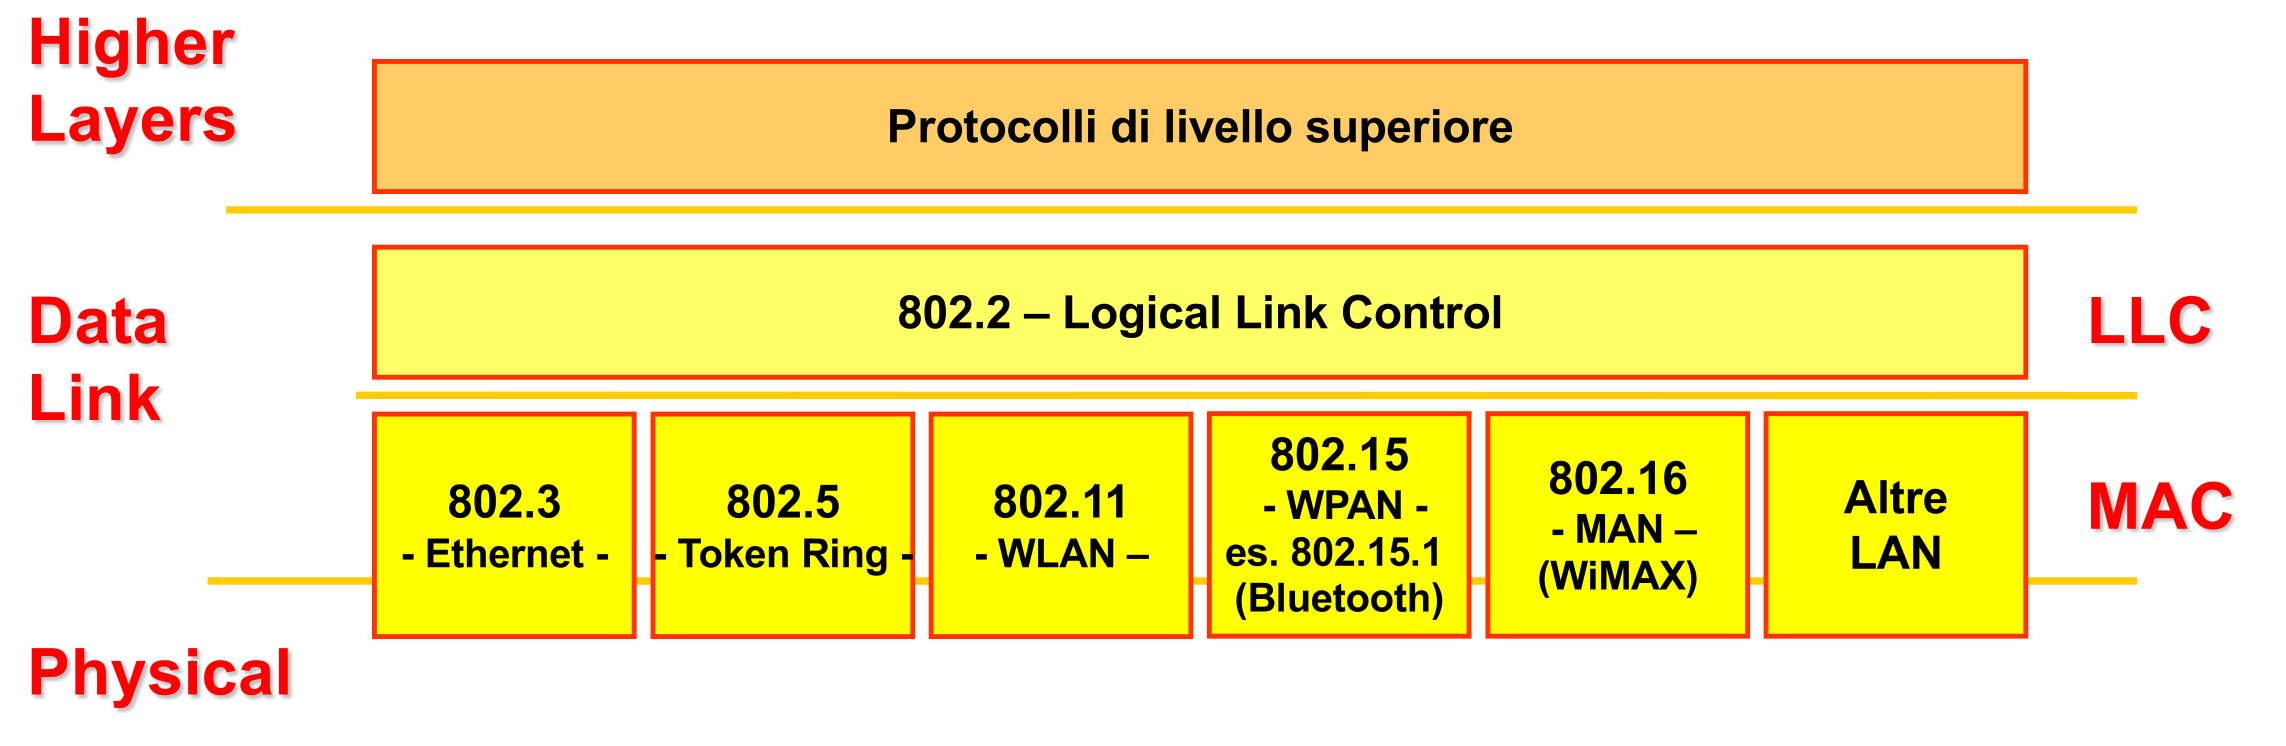
\includegraphics[width=1\textwidth]{images/ieee802.png}
    \caption{Struttura della pila ISO/OSI secondo IEEE 802}
    \label{fig:ieee802}
\end{figure}

\subsection*{IEEE 802.1}
Lo standard \texttt{IEEE 802.1} definisce le \textbf{caratteristiche generali del progetto}, comprese le specifiche per la struttura degli \textbf{indirizzi MAC}.



\subsection*{Vantaggi della suddivisione LLC/MAC}
\begin{itemize}
    \item Favorisce la \textbf{modularità} e l'interoperabilità tra diversi tipi di rete.
    \item I protocolli di livello superiore (es. IP, TCP, UDP) possono utilizzare una singola interfaccia LLC, indipendentemente dallo standard MAC sottostante.
    \item Facilita l'\textbf{evoluzione tecnologica}, permettendo l'introduzione di nuovi standard MAC senza modificare gli strati superiori.
\end{itemize}


%\subsection{Livello LLC} Il livello LLC fornisce un'interfaccia unificata tra il livello Data Link e il livello Network (es. IP), indipendentemente dallo standard MAC sottostante (Ethernet, Wi-Fi, etc.).

%\subsubsection{Frame LLC}
%spiegazione

%\begin{figure}[h!]
%    \centering
%    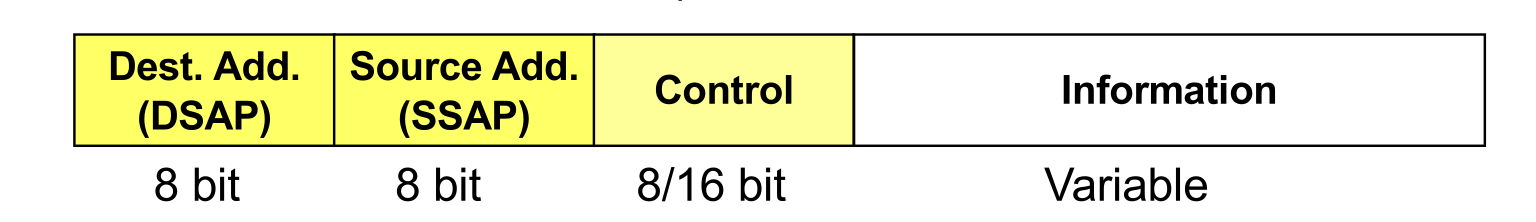
\includegraphics[width=0.7\textwidth]{images/framellc.png}
%    \caption{Struttura del frame LLC}
%   \label{fig:framellc}
%\end{figure}


%\begin{figure}[h!]
%    \centering
%    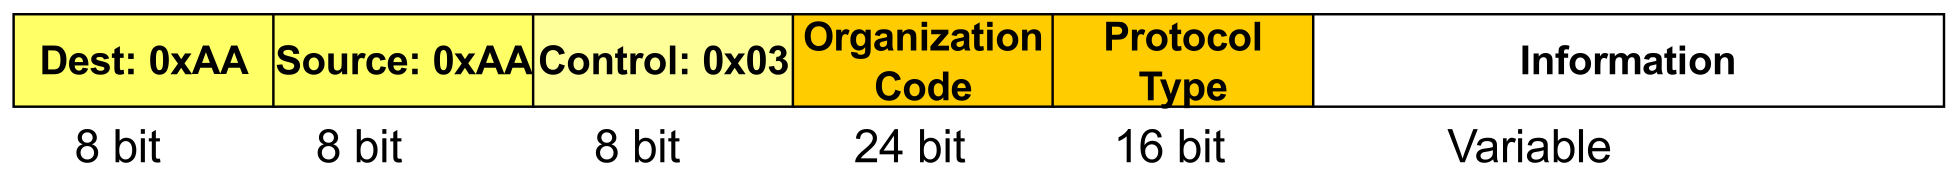
\includegraphics[width=0.7\textwidth]{images/llcsnapframe.png}
%    \caption{Struttura del frame LLC SNAP}
%    \label{fig:llcsnapframe}
%\end{figure}


%\subsection{Livello MAC}

%\begin{figure}[h!]
%    \centering
%    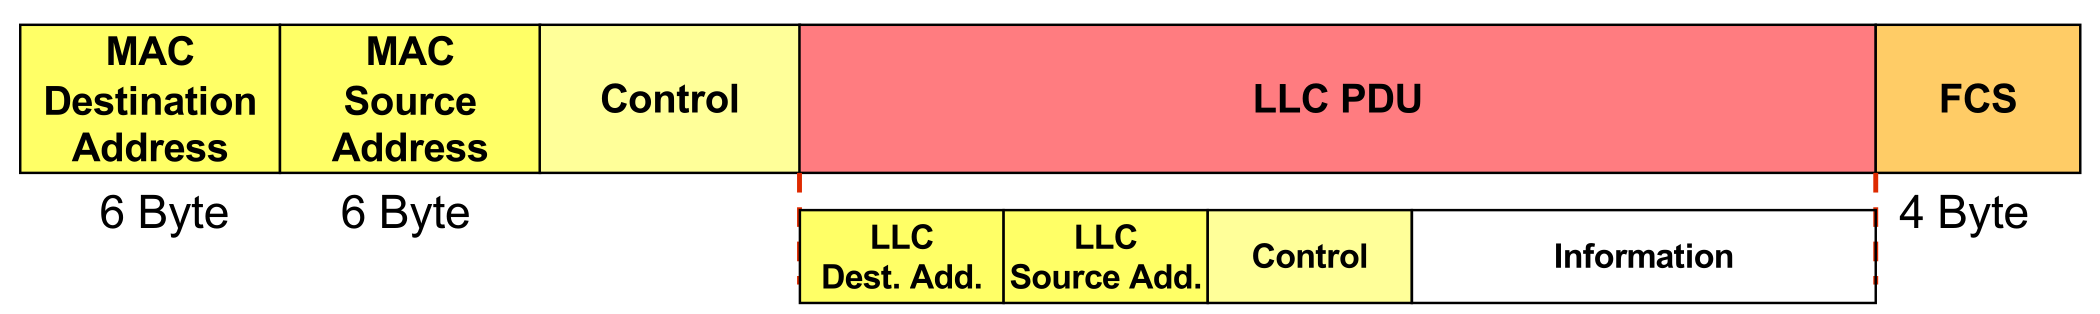
\includegraphics[width=0.7\textwidth]{images/framemac.png}
%    \caption{Struttura del frame MAC}
%    \label{fig:framemac}
%\end{figure}

%\subsubsection{MAC address}

%\subsection{Ethernet}

%\begin{figure}[h!]
%    \centering
%    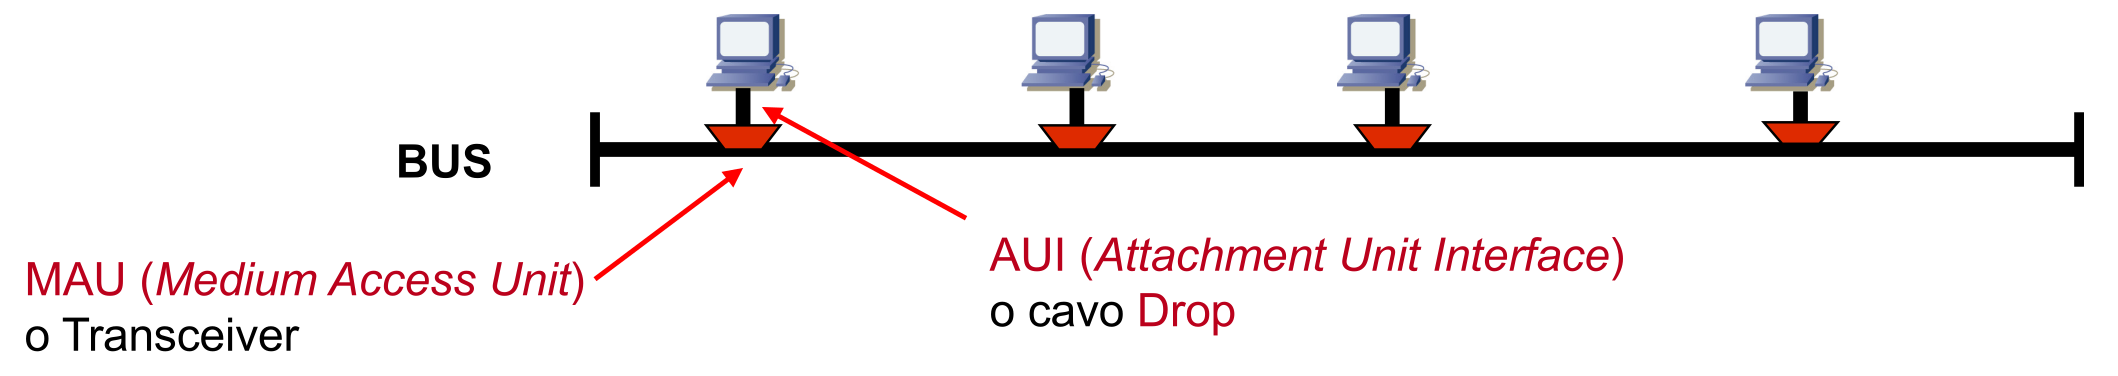
\includegraphics[width=0.7\textwidth]{images/ethernet.png}
%    \caption{Struttura del frame Ethernet}
%    \label{fig:ethernetframe}
%\end{figure}

%\subsubsection{Frame 802.3}

%\begin{figure}[h!]
%    \centering
%    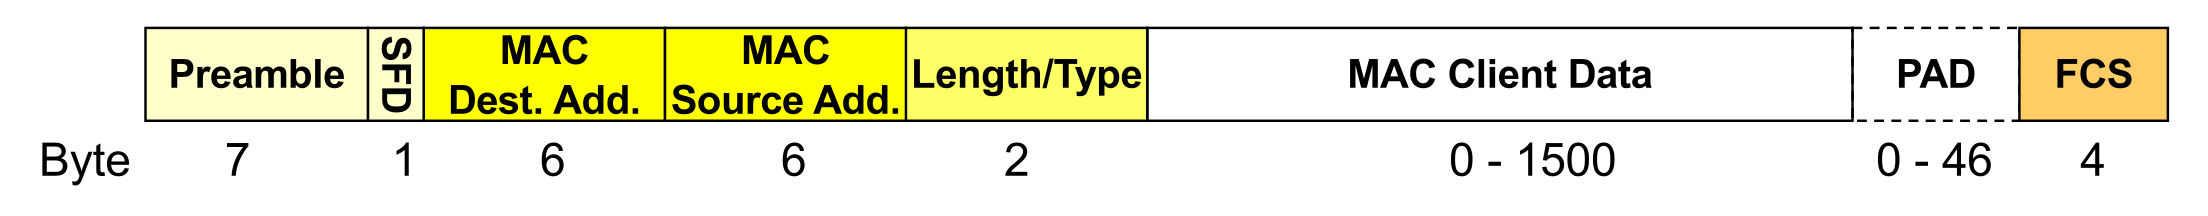
\includegraphics[width=0.7\textwidth]{images/frame8023.png}
%    \caption{Struttura del frame 802.3}
%    \label{fig:frame8023}
%\end{figure}

%\subsubsection{Inter-frame gap}
%\begin{figure}[h!]
%    \centering
%    \begin{minipage}{0.5\textwidth}
%        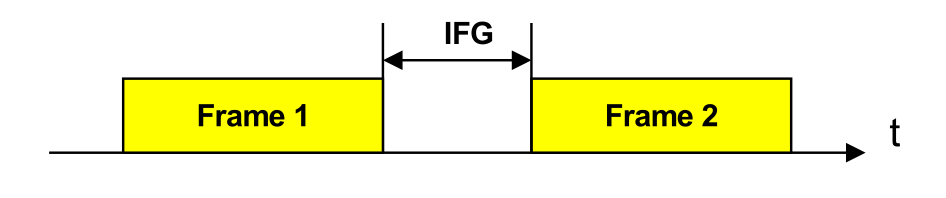
\includegraphics[width=0.9\textwidth]{images/framegap.png}
%        \caption{Inter-frame gap}
%        \label{fig:framegap}
%    \end{minipage}\hfill
%    \begin{minipage}{0.45\textwidth}
%        Spazio tra i frame.
%    \end{minipage}
%\end{figure}


%\subsubsection{Ethernet a 10 Mbit/s}

%\subsubsection{Ethernet a 100 Mbit/s}

%\subsubsection{Ethernet a 1 Gbit/s}
